% !TEX program = pdflatex
% TB-MathModeling: a multimodal, artifact-scored, feasibility-verified benchmark
% for mathematical modeling.
%
% Build:  pdflatex main && pdflatex main && pdflatex main
% (or latexmk -pdf main.tex)
%
% Files marked [TODO] need author input; everything else is populated from the repo.

\documentclass[11pt]{article}

\usepackage[utf8]{inputenc}
\usepackage[T1]{fontenc}
\usepackage{booktabs}
\usepackage{graphicx}
\usepackage{amsmath,amssymb}
\usepackage{siunitx}
\usepackage[margin=1in]{geometry}
\usepackage{hyperref}
\usepackage{multirow}
\usepackage{xcolor}
\usepackage{caption}
\usepackage{subcaption}
\usepackage{enumitem}

\newcommand{\bench}{\textsc{TB-MathModeling}}
\newcommand{\oeval}{\textsc{O-Eval}}
\newcommand{\beval}{\textsc{B-Eval}}
\newcommand{\roeval}{\textsc{Robust BO-Eval}}
\newcommand{\todo}[1]{\textcolor{red}{[TODO: #1]}}

\title{\bench{}: An Artifact-Scored, Feasibility-Verified Benchmark\\
for Multimodal LLM Agents on Mathematical Modeling}
\author{\todo{authors}\\
\todo{affiliations}}
\date{\today}

\begin{document}
\maketitle

\begin{abstract}
Large language model (LLM) agents are increasingly evaluated on tasks whose value depends on \emph{verifiable} numerical outcomes. Mathematical modeling---the practice of turning an open-ended real-world problem into assumptions, a model, a solution, and a defended recommendation---is a natural but previously unmeasured target: it is the format of the CUMCM and MCM contests, it is multimodal (official statements ship figures and spreadsheets), and its answers are only meaningful if they are \emph{both} close to a credible reference \emph{and} physically feasible.

We introduce \bench{}, a benchmark of 18 real mathematical-modeling problems (CUMCM 2023--2025 and MCM 2023--2025, problems A/B/C each year). Each task delivers the verbatim contest statement, the official attachments, and the official figures cropped from the source PDFs; the agent must produce one structured JSON artifact, scored only on the numeric core of the \emph{final} contest question against a reproduction of the corresponding outstanding (O-award) paper.

Two design choices distinguish \bench{}. First, scoring is \emph{direction-aware} and \emph{one-sided}: a metric declares whether more is better, less is better, or a target is sought, so a model is never penalised for beating the paper, while degenerate scoring bands and non-comparable reference units are handled by explicit, auditable rules. Second, feasibility is verified twice---by a programmatic gate covering all 18 tasks through six decidable invariant forms, and by a Lean~4 certificate layer that discharges 624 obligations on exact integers with no Mathlib, no \texttt{sorry}, and no (kernel-trusting) \texttt{native\_decide}. A hard gate zeroes answers that violate a stated physical constraint.

We evaluate 16 model/harness configurations, including five multimodal agents that can read the official figures. The strongest entry reaches \oeval{} 68.07\% (codex + GPT-5.5), while the cheapest near-frontier entry reaches 65.76\% at \$2.54 per 18-task run. We report per-task behaviour, a cost/robustness analysis, and three case studies (a top proprietary model, the O-award reproduction, and a low-cost open model) on representative problems. We further document---and, where the fault was ours, fix---the ways a reproduction-anchored benchmark can silently penalise correct answers, and we show how the dual feasibility layer makes the remaining failures machine-checkable rather than merely asserted.

\end{abstract}

\section{Introduction}

\subsection{Motivation}
Mathematical modeling contests (CUMCM in China, MCM/ICM internationally) ask teams to convert a deliberately under-specified real-world problem into a defensible quantitative answer within days. The deliverable is not a single number but a chain: assumptions $\rightarrow$ model $\rightarrow$ solution $\rightarrow$ sensitivity $\rightarrow$ recommendation. Two properties make this an attractive target for agent evaluation. It is \emph{quantitative}---the final question usually ends in numbers that can be checked---and it is \emph{multimodal}---official statements reference figures, and standard attachments are spreadsheets and CSVs.

Existing LLM benchmarks cover adjacent but distinct ground. Code benchmarks measure repository edits; terminal benchmarks measure command-line competence; other math benchmarks measure closed-form answers. None of them measures the modeling loop, and none of them asks whether the numbers an agent reports are \emph{feasible} under the problem's own physical constraints.

\subsection{What makes modeling hard to score}
Scoring modeling is harder than scoring code, for three reasons that shape the entire design of \bench{}:
\begin{enumerate}[leftmargin=1.4em,itemsep=2pt]
\item \textbf{There is no single ground truth.} Different teams make different assumptions. We therefore anchor on a \emph{reproduction of one outstanding paper} per task and normalise against it, rather than pretending to a canonical optimum.
\item \textbf{Anchoring creates asymmetric failure.} If the anchor is a reported number, a model that does \emph{better} than the paper can be scored worse than one that matches it. Naive distance-to-anchor scoring rewards copying and penalises improvement. \bench{} makes this direction explicit per metric and scores one-sidedly.
\item \textbf{A wrong-but-plausible answer is easy to produce.} A model can report numbers that look reasonable yet violate the problem's physics (a mirror below its allowed height, a dragon handle above its speed cap). Checking proximity to an anchor does not catch this. \bench{} adds an independent feasibility layer.
\end{enumerate}

\subsection{Contributions}
\begin{enumerate}[leftmargin=1.4em,itemsep=2pt]
\item \textbf{A multimodal, artifact-scored benchmark of 18 real modeling problems.} Verbatim statements, official attachments, and 21 figures cropped from the source PDFs; one structured JSON artifact per task; scoring restricted to the numeric core of the final contest question.
\item \textbf{Direction-aware, one-sided scoring with auditable edge-case rules.} Per-metric semantic direction (\texttt{higher\_is\_better} / \texttt{lower\_is\_better} / \texttt{target\_value} / \texttt{exact\_value}); three reported metrics (\oeval{}, \beval{}, \roeval{}); explicit rules for degenerate scoring bands and for reference values whose units are not pinned by the schema, together with contract tests that lock the two properties down.
\item \textbf{A two-layer feasibility verification design.} A programmatic gate covering 18/18 tasks via six decidable invariant forms, and a Lean~4 certificate layer of 624 kernel-checked obligations; we characterise precisely which feasibility questions each layer can and cannot answer.
\item \textbf{An empirical study of 16 model/harness configurations}, including five multimodal agents, with per-task behaviour, cost/robustness analysis, and three case studies. We additionally document systematic scoring pitfalls that we found and fixed, and quantify their effect on the leaderboard.
\end{enumerate}

\subsection{Summary of findings}
The best entry, codex + GPT-5.5 (xhigh), reaches \oeval{} 68.07\% and \roeval{} 23.62\% at \$99.37 per run. A low-cost open model, opencode + DeepSeek~V4.1~Flash, reaches 65.76\% / 18.36\% at \$2.54---roughly a 39$\times$ cost gap for 2.3 points of \oeval{}. Raising a model's thinking tier from its default to its maximum does \emph{not} help (54.93\% vs.\ 65.76\% for the same model). Most residual failures are attributable to reference-value scale/scope mismatches rather than to modeling errors, a finding we quantify and partially repair.

\section{Related Work}

\todo{fill citations; the paragraph claims below are the intended framing}

\paragraph{LLM agent benchmarks.}
Software-engineering and terminal agents are measured by repository tasks (SWE-bench~\cite{TODO-swebench}) and by end-to-end command-line tasks (Terminal-Bench~\cite{TODO-terminalbench}); general assistants are measured by tool-use suites (GAIA~\cite{TODO-gaia}, $\tau$-bench~\cite{TODO-taubench}). These capture tool use and code editing but do not score a modeling artifact, and they do not attach a feasibility contract to the answer.

\paragraph{Mathematical and optimization reasoning.}
Closed-form math benchmarks (competition mathematics~\cite{TODO-math}, frontier research mathematics~\cite{TODO-frontiermath}, formal-to-natural proving~\cite{TODO-minif2f}) measure deduction, not modeling. Operations-research datasets (e.g.\ NL4OPT~\cite{TODO-nl4opt}) parse word problems into solvers; they do not require assumptions, sensitivity, or a defended recommendation. Machine-learning engineering benchmarks (MLE-bench~\cite{TODO-mlebench}) are the closest in spirit but are scored by leaderboard position rather than by a physical feasibility contract.

\paragraph{Formal verification in evaluation.}
Interactive theorem provers such as Lean~4~\cite{TODO-lean4} with Mathlib~\cite{TODO-mathlib} have been used to certify competition and research mathematics (e.g.\ AlphaProof~\cite{TODO-alphaproof}). Using a prover not to \emph{find} answers but to \emph{audit} a benchmark's feasibility decisions is, to our knowledge, new: our Lean layer re-proves the invariants that the programmatic gate checks, so the audit itself becomes machine-checkable.

\paragraph{Multimodal agents.}
Vision-language agents are increasingly given screenshots and diagrams. \bench{} contributes a setting where figures are load-bearing---they are cropped from the official PDFs and referenced inline in the statement---and where we can compare text-only and multimodal harnesses on the same tasks.

\paragraph{Reproduction-anchored scoring.}
Anchoring on a published solution is standard in numerical-answer benchmarks. We show that this creates three specific, previously under-reported hazards---direction asymmetry, degenerate bands, and unpinned units---and give auditable rules and contract tests for each.

\section{The \bench{} Benchmark}
\label{sec:benchmark}

\subsection{Task selection and sources}
\bench{} comprises \textbf{18 tasks}: the A, B, and C problems of CUMCM and of MCM for each of 2023, 2024, and 2025. The two contests are complementary in style---CUMCM problems are engineering/optimization-heavy and stated in Chinese; MCM problems are modeling-flavored and stated in English---and taking all three problems of each year covers the standard ``A = physical/engineering, B = data/optimization, C = data-science'' split without cherry-picking.

Everything is derived from the official contest material. Problem statements are taken from the local corpus (CUMCM: \texttt{cumcm/problems/\{year\}/\{X\}.md}; MCM: \texttt{mcm/problems/\{year\}/\{X\}.md}), and the official attachments (PDFs, \texttt{.xlsx}, \texttt{.csv}) are mirrored verbatim. Table~\ref{tab:tasks} lists the 18 tasks and the outstanding paper each one is anchored to.

\begin{table}[t]
\centering
\small
\caption{The 18 \bench{} tasks and their O-award anchors. ``Final Q'' is the contest question whose numeric core is scored; oracle coverage is 18/18.}
\label{tab:tasks}
\begin{tabular}{@{}lllll@{}}
\toprule
Slug & Contest & Topic & Final Q & O-award \\
\midrule
\texttt{cumcm-2023-a-heliostat-field}   & CUMCM 2023 A & Heliostat field design        & Q3 & A175 \\
\texttt{cumcm-2023-b-multibeam-lines}   & CUMCM 2023 B & Multibeam survey lines        & Q4 & B226 \\
\texttt{cumcm-2023-c-vegetable-pricing} & CUMCM 2023 C & Vegetable pricing/replenish   & Q4 & C050 \\
\texttt{cumcm-2024-a-dragon-dance}      & CUMCM 2024 A & Bench-dragon kinematics       & Q5 & A016 \\
\texttt{cumcm-2024-b-production-decision}& CUMCM 2024 B & Production decisions          & Q4 & B159 \\
\texttt{cumcm-2024-c-crop-planting}     & CUMCM 2024 C & Crop-planting strategy        & Q1 & C038 \\
\texttt{cumcm-2025-a-smoke-screen}      & CUMCM 2025 A & UAV smoke-screen strategy     & Q5 & A196 \\
\texttt{cumcm-2025-b-sic-thickness}     & CUMCM 2025 B & SiC epi-layer thickness       & Q3 & B157 \\
\texttt{cumcm-2025-c-nipt}              & CUMCM 2025 C & NIPT timing / abnormality     & Q4 & C023 \\
\texttt{mcm-2023-a-plant-community}     & MCM 2023 A & Drought plant communities     & final & 2309229 \\
\texttt{mcm-2023-b-maasai-mara}         & MCM 2023 B & Maasai Mara land use          & final & 2315379 \\
\texttt{mcm-2023-c-wordle}              & MCM 2023 C & Predicting Wordle results     & final & 2307946 \\
\texttt{mcm-2024-a-lamprey}             & MCM 2024 A & Sex ratios / resource supply  & final & 2407093 \\
\texttt{mcm-2024-b-submersible-search}  & MCM 2024 B & Submersible search            & Q4 & 2419984 \\
\texttt{mcm-2024-c-tennis-momentum}     & MCM 2024 C & Momentum in tennis            & Q5 & 2401298 \\
\texttt{mcm-2025-a-stair-wear}          & MCM 2025 A & Stair wear / footfall         & Q8 & 2501909 \\
\texttt{mcm-2025-b-juneau-tourism}      & MCM 2025 B & Sustainable tourism (Juneau)  & Q3 & 2504448 \\
\texttt{mcm-2025-c-olympic-medals}      & MCM 2025 C & Olympic medal models          & final & 2505964 \\
\bottomrule
\end{tabular}
\end{table}

\subsection{Construction pipeline}
Each task is generated by a build script that is reproducible from the source corpus. The generated directory has a fixed shape:
\begin{itemize}[leftmargin=1.4em,itemsep=1pt]
\item \texttt{instruction.md} --- the prompt. It contains the verbatim contest statement, each cited figure embedded inline, a note giving the in-container figure paths, and a ``Required Benchmark Artifact'' section naming the output file. It ends with the time limit.
\item \texttt{environment/} --- the agent container: a Dockerfile (\texttt{python:3.12-slim} plus a fixed scientific-Python environment) and \texttt{data/}, holding \texttt{problem.md}, \texttt{output\_schema.json}, \texttt{source\_manifest.json}, an \texttt{attachments/} flat mirror with an \texttt{INDEX.md}, a \texttt{repo/} full-path mirror of the original corpus, and any \texttt{figures/}.
\item \texttt{tests/} --- the verifier (a separate container): \texttt{test.sh}, \texttt{test\_outputs.py}, \texttt{score\_result.py}, plus the scoring panel \texttt{score\_config.json}, the anchor \texttt{expected\_result.json}, and auxiliary checks.
\item \texttt{solution/} --- the oracle: \texttt{solve.sh} and \texttt{oracle/}, which contains a runnable reproduction of the anchored O-award paper.
\end{itemize}

\paragraph{Figures are load-bearing.} For problems whose statements cite figures, the figures are cropped from the official PDF---artwork plus its own caption, without surrounding prose---and delivered both inline in the statement and at stable container paths. \textbf{21 unique figures} across 6 tasks (CUMCM 18, MCM 3) are delivered this way; the remaining 12 tasks have no figure. This matters because a text-only agent cannot see them (Figure~\ref{fig:official-fig}), which is exactly what the multimodal comparison in Section~\ref{sec:results} exploits.

\begin{figure}[t]
\centering
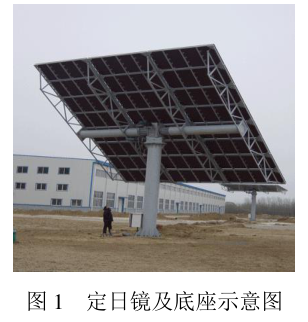
\includegraphics[width=0.62\linewidth]{figures/heliostat_statement_fig1.png}
\caption{An official statement figure, cropped from the CUMCM 2023 A PDF (artwork plus its own caption, without surrounding prose) and delivered inline in the prompt. 21 such figures across 6 tasks are load-bearing: a text-only agent cannot read them.}
\label{fig:official-fig}
\end{figure}

\paragraph{No train/test split.} \bench{} is a pure evaluation set. There is no training partition, no held-out split, and no difficulty tiering: the 18 tasks are evaluated uniformly. This is deliberate for a benchmark of this kind and is stated explicitly in Appendix~\ref{app:dataset}.

\subsection{The artifact contract}
The single scored object is one JSON file per task. Its expected shape is shipped to the agent as \texttt{output\_schema.json} (field names and types only, no values), and the agent is told the exact path (\texttt{/root/results/<slug>\_result.json}). Supplementary CSV/XLSX/PNG artifacts may be written but are not scored. Restricting scoring to a schema-constrained JSON is what makes an automated, reproducible score possible at all; the cost is that the agent must map a free-form modeling effort onto a small set of named numeric fields, which we revisit in Section~\ref{sec:analysis}.

\subsection{Oracle anchors}
Each task is anchored to one outstanding (O-award) paper, re-implemented as a runnable script that reads the official attachments and emits the same artifact JSON. The reproduction is used as the normalization endpoint (\oeval{} $=100\%$), and its per-metric values initialize the scoring panel. Oracle coverage is \textbf{18/18}: every task ships \texttt{solution/oracle/} and an \texttt{expected\_result.json}.

We are explicit about two consequences. First, an anchor is a \emph{reproduction} of one team's choices, not an optimum; Section~\ref{sec:scoring} explains how scoring is designed so that beating the anchor is not punished. Second, reproductions can themselves be wrong. We found and corrected one such case---the dragon-dance final answer---and we treat anchor provenance as a first-class field (each reproduction records its paper id, OCR/PDF source, and a \texttt{reproduction\_scope}). Appendix~\ref{app:baselines} lists the anchors; Section~\ref{sec:analysis} quantifies the anchor-related failure modes.

\section{Scoring: Direction-Aware, One-Sided, Auditable}
\label{sec:scoring}

Scoring a modeling artifact against a reproduced paper is a comparison of numbers, but a naive distance metric silently rewards copying and punishes improvement. \bench{} therefore scores each task through a \emph{per-metric panel} with an explicit semantic direction, and aggregates at three levels.

\subsection{Per-metric scoring}
\label{sec:per-metric}
Each task's \texttt{score\_config.json} declares a small panel of metrics (2--6 per task; 62 declared metrics in total, of which 61 are scored), each with a path into the artifact JSON, an anchor value $O$, a direction, and a weight. Let $\mathrm{actual}$ be the model's reported value (after a percent-to-fraction hook: a unit-interval, percent-like metric reported in $(10,100]$ is divided by 100).

\textbf{Directions.} A metric is one of \texttt{higher\_is\_better}, \texttt{lower\_is\_better}, \texttt{target\_value} (closest to $O$ wins), or \texttt{exact\_value} (integer/discrete match). Direction is set per metric from the modeling semantics, not from the number's sign.

\textbf{Two normalisation modes.} A metric either uses a \emph{legacy target-distance} scale
\[
\mathrm{scale} = \max\bigl(\mathrm{abs\_scale},\; r\cdot\max(|O|,1)\bigr),\qquad r = 0.12,\ \mathrm{abs\_scale}=10^{-6},
\]
or a \emph{baseline-to-outstanding endpoint} band $B = |O - b|$ (where $b$ is a baseline value), used by the three endpoint-style tasks.

\textbf{One-sided reward.} For directional metrics the reward is asymmetric by construction:
\begin{align}
\texttt{higher\_is\_better}:&\quad
\begin{cases}
1 + \log\!\bigl(1 + (\mathrm{actual}-O)/\mathrm{scale}\bigr), & \mathrm{actual}\ge O,\\[2pt]
\dfrac{1}{1 + (O-\mathrm{actual})/\mathrm{scale}}, & \mathrm{actual}< O,
\end{cases}\\
\texttt{lower\_is\_better}:&\quad \text{symmetric in } O-\mathrm{actual},\\
\texttt{target\_value}:&\quad \dfrac{1}{1 + |\mathrm{actual}-O|/\mathrm{scale}},\qquad
\texttt{exact\_value}:\quad \mathbb{1}[\mathrm{actual}=O].
\end{align}
The key property is that \emph{meeting or beating the anchor never scores below 1.0}: a model that improves on the paper is not punished. In endpoint mode the same asymmetry holds, with the below-anchor branch replaced by $\mathrm{clamp}_{[0,1]}\bigl((\mathrm{actual}-b)/B\bigr)$.

\subsection{Edge-case rules, made explicit}
\label{sec:edge-rules}
Three failure modes of anchor-based scoring are common enough to deserve named, testable rules.

\paragraph{(i) Degenerate bands.} When an endpoint band is narrower than 2\% of the value magnitude, it cannot discriminate: the paper's own baseline sits at 0 and so does every other answer. We widen such a band to 5\% (overridable per metric via \texttt{min\_rel\_band}); a merely narrow-but-sane band is left exactly as configured. This rule changed exactly one cell (stair-wear, whose band was $72.67\!\to\!73.52$, i.e.\ 1.2\%).

\paragraph{(ii) Non-comparable reference units.} Some anchors report an \emph{arbitrary raw index} the schema never defines a unit for (e.g.\ a host-fish population index of 1080). A model that reports the same quantity normalised to $[0,1]$ is not demonstrably wrong. Rather than auto-rescaling (which would also pass real errors), such metrics are \emph{dropped from the panel for every model and for the oracle alike}, keeping the comparison like-for-like. This rule is keyed only on the metric configuration, so it is identical for all submissions.

\paragraph{(iii) Prompt/reference cardinality mismatch.} When the prompt asks for a fixed number of items but the reproduction emits more (a country--sport recommendation list of 4 rows where the prompt asks for three), the surplus row is excluded rather than counted as missing.

\paragraph{Validity zeroing (distinct from exclusion).} A metric whose reported value is out of its declared domain---a correlation outside $[-1,1]$, a unit-interval quantity outside $[0,1]$, a negative count or a non-positive physical quantity---has its reward set to zero, with the reason recorded.

\subsection{Aggregation}
Let $R=\sum_m w_m r_m / \sum_m w_m$ be the weighted panel score (\emph{direction-aware raw}) of a submission on a task, and let $F$ and $O$ be the same panel applied to the flash baseline and to the oracle reproduction. Then
\begin{align}
\oeval &= \min\bigl(1,\ \max(0,\ R / O)\bigr) \quad\text{per task, averaged over 18 tasks},\\
\beval &= R - F \quad\text{(raw units; reported as percentage points)},\\
\roeval &= \begin{cases}
\mathrm{clip}\bigl((R-F)/(O-F),\,-1,\,+1\bigr), & O-F \ge 0.10,\\[2pt]
\mathrm{clip}\bigl(R-F,\,-0.10,\,+0.10\bigr), & \text{otherwise},
\end{cases}
\end{align}
with any missing or non-scoreable artifact assigned $\roeval=-1$. \oeval{} is the headline absolute score (100\% $=$ the O-award reproduction's raw panel level, overshoots capped). \roeval{} is a robustness diagnostic that compensates for tiny or saturated gaps, so that a leaderboard is not driven by ratio outliers.

\subsection{Hard gate}
\label{sec:hard-gate}
If a submission fails the feasibility gate of Section~\ref{sec:verification}, its panel score is not merely reduced: the whole task's raw is set to $0$ (\oeval{}$\,=0\%$) and \roeval{} to $-1$. The gate has two sources: programmatic checks (all 18 tasks) and a small set of hand-adjudicated whole-task penalties (4 rules) for constraints that need an independent replay. Section~\ref{sec:analysis} shows how many cells this affects and why.

\subsection{Contract tests}
Two properties are enforced by \texttt{scripts/test\_scoring\_contracts.py}, because they are exactly the ones that break silently:
\begin{itemize}[leftmargin=1.4em,itemsep=1pt]
\item \textbf{Oracle self-consistency}: every task's reproduction must score a panel of exactly $1.0$. If it does not, the anchors or schema paths are wrong and every downstream \oeval{} is meaningless.
\item \textbf{One-sidedness}: on \texttt{higher\_is\_better}, a result at or above the anchor is never a failure (and symmetrically for \texttt{lower\_is\_better}).
\end{itemize}

\section{Feasibility Verification: Two Layers}
\label{sec:verification}

Proximity to an anchor does not imply that an answer is \emph{physically admissible}. A submission can match a reference value on one field while violating a stated constraint on another, or can report numbers that are internally contradictory. \bench{} verifies feasibility independently of scoring, in two layers with different trust bases.

\subsection{Layer 1: a programmatic gate over six decidable forms}
Every task registers one feasibility check. The gate is a registry covering \textbf{18/18} tasks, and every hard-error branch it can raise falls into one of six decidable forms:

\begin{table}[h]
\centering
\small
\caption{The six decidable invariant forms covering all 18 tasks' hard-error branches.}
\label{tab:invariants}
\begin{tabular}{@{}ll@{}}
\toprule
Form & Example obligation \\
\midrule
domain / range        & probability $\in[0,1]$; thickness $\in(0,500]\,\mu$m \\
integer / binary      & decision bits $\in\{0,1\}$; counts are integers \\
ordering              & $q_{95}\ge$ mean; peak users $\ge$ spread average; interval low $\le$ high \\
exact identity        & area $=$ count $\times$ width $\times$ height; union $\le \sum$ parts \\
finite-domain         & decision-bit count $\in\{16,17\}$; case ids $=\{1..6\}$ \\
partition / sum       & four land-use counts sum to the declared grid \\
\bottomrule
\end{tabular}
\end{table}

Checks come in two styles: \emph{structural/domain bounds} (rates, correlations, probabilities, nonnegative counts, distributions summing to 100, peak $\ge$ average) and \emph{constraint replay} (heliostat rated power $\ge 60$~MW and installation height $\in[2,6]$~m; dragon-dance head speed $\times$ amplification ratio $\le 2$~m/s; crop-planting demand-capped revenue ceiling; smoke-screen union duration $\le$ sum of parts).

Three contracts keep the gate honest, enforced by \texttt{test\_feasibility\_checks.py}:
\textbf{coverage} (a task cannot ship ungated), \textbf{oracle self-consistency} (the O-award reference must pass its own check---a gate that rejects the human solution is wrong by construction), and \textbf{discrimination} (synthetic and real-field violations must be rejected for the right reason; an empty artifact must warn, not hard-fail).

\paragraph{Hand adjudication.} Four constraints require an independent replay rather than a field check and are recorded as whole-task penalties: a heliostat design whose tail mirror sits below the 2~m minimum; a smoke-screen plan whose independent replay gives zero coverage; a tourism answer whose acceptance index and sustainability score are on the wrong scale; and an Olympic coach-effect answer whose scored recommendations are degenerate.

\subsection{Layer 2: Lean certificates}
The programmatic gate is only as trustworthy as its code. Layer 2 re-proves the same invariants as Lean~4 theorems, so the audit itself becomes machine-checkable.

\textbf{Scale and scope.} The layer generates \textbf{624 obligations across all 18 tasks}, evaluated against the real saved artifacts. Every obligation is discharged by \texttt{decide} (exact-integer decision) or \texttt{omega} (integer linear arithmetic). \textbf{No Mathlib is used}: because the checked propositions are decidable on exact integers, Lean core suffices, and a clean build completes in about a second.

\textbf{Exactness.} Values are scaled to exact integers before comparison (rates $\times1000$, money $\times1$), so there is no floating-point tolerance anywhere. The one tolerance that exists---for a unit-like composite index---is \emph{declared} in the predicate (\texttt{InIndex scale tol}) rather than hidden in the code, because ``how much tolerance is allowed'' is itself part of the modeling assumption being audited.

\textbf{Trust audit.} \texttt{\#print axioms} on every certificate reports only \texttt{[propext, Quot.sound]} (Lean's standard classical logic) or no axioms at all. Crucially, there is \textbf{no \texttt{sorryAx}} (an admitted gap) and \textbf{no \texttt{native\_decide}} (which would trust the compiler via \texttt{Lean.ofReduceBool} rather than the kernel). The layer is grep-checked for both; a certificate that only ``runs clean'' is not accepted.

\textbf{Discrimination.} A checker that cannot fail is worthless. A discrimination suite mutates one numeric leaf at a time and requires the build to break \emph{and} to cite the mutated field. \textbf{10 mutations across all six forms}---out-of-range probability, out-of-range correlation, reversed ordering (discount profit below wasted-surplus profit), a violated exact identity (head speed $\times$ ratio $\ne$ 2~m/s), non-positive thickness, reversed interval, a non-binary decision bit, a negative acceptance index, a $q_{95}$ below its mean, and a zero species count---are all rejected, each pointing at its own field.

\textbf{What the layer upgrades.} Two soft warnings in the programmatic gate become proofs. A tourism artifact whose acceptance index is 85.098 is \emph{refuted} for the unit convention and shown to fit the percent convention; its sustainability score 118.362 is shown to fit \emph{neither} under any tolerance within the declared 5\% budget---so ``just widen the tolerance'' is not an escape. A crop-planting profit is shown to lie strictly inside the per-plot/aggregate demand-cap interpretation gap, so the verdict rests on a declared reading rather than on arithmetic.

\subsection{What verification can and cannot do}
\label{sec:abc}
The two layers cover two of three feasibility questions, and we state the boundary explicitly, because conflating them would overclaim.

\begin{table}[h]
\centering
\small
\caption{Three layers of feasibility. Both our layers cover A and B; C requires formalising physics.}
\label{tab:abc}
\begin{tabular}{@{}lp{6.4cm}l@{}}
\toprule
Layer & Content & Covered by \\
\midrule
A --- unit / range & probability $\in[0,1]$, thickness $>0$, percentages in range & gate + Lean \\
B --- internal consistency & area $=$ count $\times$ w $\times$ h, partitions sum, union $\le$ parts & gate + Lean \\
C --- external physical truth & does this mirror field really produce 60~MW? & neither (replay / hand) \\
\bottomrule
\end{tabular}
\end{table}

Lean proves ``the reported value is 60.0 and $60.0\ge60$''; it does not prove ``the field produces 60~MW''. The latter would require formalising optics and geometry, which is out of scope. Likewise, the layer's strength is bounded by \emph{witness completeness}: it can only check what the artifact exposes. Where a task reports only summary scalars, the layer inherits the same blind spot---so three obligations are \emph{skipped and reported} rather than silently satisfied (a missing overlap field, a null declared grid count, and a recommendation-count interpretation difference). Making these visible is itself part of the design: an audit that hides its gaps is not an audit.

\section{Experimental Setup}
\label{sec:setup}

\subsection{Models and harnesses}
We evaluate \textbf{16 configurations} spanning proprietary and open models, three agent harnesses, and multiple reasoning tiers. Because the tasks ship figures, we distinguish \emph{multimodal} entries (the harness can open the cropped PNGs) from text-only entries (the \texttt{terminus-2} agent has no image channel). Table~\ref{tab:configs} summarises the roster; full commands and configuration are in Appendix~\ref{app:settings}.

\begin{table}[t]
\centering
\small
\caption{The 16 evaluated configurations. ``MM'' marks multimodal harnesses. Cost is the normalized 18-task, one-attempt estimate.}
\label{tab:configs}
\begin{tabular}{@{}llcccc@{}}
\toprule
Entry & Model & Harness & Tier & MM & Cost (USD) \\
\midrule
codex + gpt-5.5 xhigh            & \texttt{openai/gpt-5.5}            & codex CLI       & xhigh & \checkmark & 99.37 \\
Qwen3.8-27B-FP8 thinking         & \texttt{qwen/qwen3.8-27b}          & terminus-2      & thinking & & 28.18 \\
opencode + deepseek-flash        & \texttt{deepseek/deepseek-v4.1-flash} & opencode CLI & high (default) & \checkmark & 2.54 \\
Tencent Hy4 Preview              & \texttt{tencent/hy4-preview}       & terminus-2      & default & & 14.54 \\
GPT-5.6 SOL high                 & \texttt{openai/gpt-5.6-sol}        & terminus-2      & high & & 8.90 \\
claude-code + Fable 5.1          & \texttt{claude-fable-5-1}          & claude-code CLI & max & \checkmark & 272.80 \\
GPT-5.6 SOL xhigh                & \texttt{openai/gpt-5.6-sol}        & terminus-2      & xhigh & & 14.73 \\
v4 pro                           & \texttt{deepseek/deepseek-v4-pro}  & terminus-2      & default & & 5.55 \\
GLM-5.3                          & \texttt{z-ai/glm-5.3}              & terminus-2      & default & & 38.30 \\
Kimi K3                          & \texttt{moonshotai/kimi-k3}        & terminus-2      & default & & 26.68 \\
opencode + deepseek-flash (max)  & \texttt{deepseek/deepseek-v4.1-flash} & opencode CLI & max & \checkmark & 2.78 \\
codex + GPT-6 Astra              & \texttt{gpt-6-astra}               & codex CLI       & max & \checkmark & 246.41 \\
GLM-5.3-Flash (ox-alpha)         & \texttt{z-ai/glm-5.3-flash}        & terminus-2      & default & & 2.91 \\
v4 flash baseline                & \texttt{deepseek/deepseek-v4-flash-0731} & terminus-2 & default & & 0.68 \\
Qwen3.8 Flash (Bailian)          & \texttt{qwen/qwen3.8-flash}        & terminus-2      & default & & 8.81 \\
Gemini 3.7 Flash high            & \texttt{google/gemini-3.7-flash}   & terminus-2      & high & & 6.15 \\
\bottomrule
\end{tabular}
\end{table}

Two entries deserve notes. \textbf{opencode + deepseek-flash (max)} is the same model and harness as the high entry, differing only in the thinking tier (\texttt{variant=max} vs.\ the default \texttt{high}); it is a controlled tier comparison, not a separate model. \textbf{codex + GPT-6 Astra} and \textbf{claude-code + Fable 5.1} are third-party runs (independent operators, Modal, October 2026) on the same task revision; we re-scored their artifacts with \emph{our} scorer and current anchors so that all 16 rows share one scoring definition.

\subsection{Prompt design}
The prompt is the task's \texttt{instruction.md}, passed verbatim by the harness. It contains the original contest statement, the cited figures inline, and a fixed ``Required Benchmark Artifact'' block naming the output path. \texttt{terminus-2} prepends a generic command-line system prompt; \texttt{codex} and \texttt{opencode} receive the statement as their positional prompt. Appendix~\ref{app:prompts} reproduces the template and the exact per-harness commands.

\emph{Version caveat.} The \texttt{instruction.md} files were revised after some trials were recorded (figure-path notes added; one statement re-sourced). The paper therefore describes the prompt as delivered in the recorded trials, not as the file reads today; the captured command lines in each \texttt{trial.log} are authoritative.

\subsection{Environment}
Tasks run in Docker containers under harbor~0.14.0. Each task's agent container is \texttt{python:3.12-slim} with a fixed scientific stack (NumPy 2.0.2, pandas 2.2.2, SciPy 1.14.1, scikit-learn 1.5.2, Matplotlib 3.9.2, openpyxl 3.1.5, xlrd 2.0.1) and \texttt{MPLBACKEND=Agg}. Resource limits are 2 CPUs, 8~GB memory, 20~GB storage, no GPU; the agent timeout is 4~hours, the verifier timeout 180~s. \textbf{Internet is disabled} (\texttt{allow\_internet=false}); model traffic is routed through a local retry proxy, so an agent cannot fetch solutions or install packages at runtime. The verifier runs in a \emph{separate} container that only has pytest. Full details are in Appendix~\ref{app:environment}.

\subsection{Protocol and statistics}
Each model is evaluated on all 18 tasks with a single attempt (\texttt{n\_attempts=1}, no retries), so the main results are single-run. Two consequences are reported honestly rather than papered over: (i) we do not select ``the best run''---a single run is a single run; and (ii) we cannot report multi-seed mean$/$std. The one task with repeated attempts is the dragon-dance problem, run four times per model as a consistency probe; the four answers were identical to machine precision (\texttt{mean}=1.246266, \texttt{std}=$4.6\times10^{-16}$). We report that as evidence of determinism on a numerically well-posed task, not as a variance estimate.

\section{Results}
\label{sec:results}

\subsection{Main result: 16 configurations on 18 tasks}
Table~\ref{tab:main} reports the primary leaderboard. \oeval{} is the absolute oracle-normalised score (100\% $=$ the O-award reproduction), \beval{} the raw gain over the flash baseline in percentage points, and \roeval{} the gap-compensated robustness score.

\begin{table}[t]
\centering
\small
\caption{Main leaderboard, 18 tasks. Rows sorted by \oeval{}. ``Art.'' is the number of tasks with a scoreable artifact (out of 18). Cost is USD for one 18-task pass.}
\label{tab:main}
\begin{tabular}{@{}lccccr@{}}
\toprule
Model / harness & Art. & \oeval{} & \beval{} & \roeval{} & Cost \\
\midrule
codex + gpt-5.5 xhigh          & 18 & 68.07\% & +10.82\,pp & 23.62\% & \$99.37 \\
Qwen3.8-27B-FP8 thinking       & 18 & 65.81\% & +8.25\,pp  & 22.41\% & \$28.18 \\
opencode + deepseek-flash      & 18 & 65.76\% & +15.88\,pp & 18.36\% & \$2.54 \\
Kimi K3                        & 18 & 65.36\% & +16.20\,pp & 21.41\% & \$26.68 \\
Tencent Hy4 Preview            & 18 & 64.78\% & +15.83\,pp & 16.50\% & \$14.54 \\
GPT-5.6 SOL high               & 18 & 63.67\% & +14.44\,pp & 16.12\% & \$8.90 \\
claude-code + Fable 5.1        & 18 & 62.62\% & +10.61\,pp & 20.22\% & \$272.80 \\
GLM-5.3                        & 18 & 60.43\% & $-9.61$\,pp & 12.97\% & \$38.30 \\
GPT-5.6 SOL xhigh              & 17 & 60.40\% & $-4.81$\,pp & 9.79\%  & \$14.73 \\
v4 pro                         & 18 & 58.62\% & $-6.83$\,pp & 12.30\% & \$5.55 \\
GLM-5.3-Flash (ox-alpha)       & 18 & 57.93\% & $-3.14$\,pp & 10.13\% & \$2.91 \\
Qwen3.8 Flash (Bailian)        & 18 & 55.31\% & $-11.74$\,pp & 4.86\% & \$8.81 \\
opencode + deepseek-flash (max)& 17 & 54.93\% & $-13.26$\,pp & 12.74\% & \$2.78 \\
v4 flash baseline              & 17 & 54.59\% & +0.00\,pp & 0.00\% & \$0.68 \\
codex + GPT-6 Astra            & 18 & 52.85\% & $-0.84$\,pp & 16.03\% & \$246.41 \\
Gemini 3.7 Flash high          & 15 & 51.99\% & $-12.55$\,pp & $-4.91$\% & \$6.15 \\
\bottomrule
\end{tabular}
\end{table}

\textbf{Findings.}
\begin{enumerate}[leftmargin=1.4em,itemsep=2pt]
\item \textbf{Frontier capability is compressed, cost is not.} The top five entries fall within 3.3 \oeval{} points (68.07\%--64.78\%), yet the cheapest of them costs \$2.54 and the most expensive \$99.37---a $39\times$ gap for 2.3 points between the first and third rows. On this benchmark, spend buys very little beyond a certain point.
\item \textbf{Thinking tier is not monotone.} opencode + deepseek-flash with the maximum tier scores 54.93\%, \emph{below} its default-tier counterpart at 65.76\%, at higher cost. A more expensive deliberative setting hurt this model on these tasks.
\item \textbf{Newer flagship labels do not imply higher scores here.} codex + GPT-6 Astra (52.85\%) and claude-code + Fable 5.1 (62.62\%)---both recent, both multimodal, and together costing \$519---land below the cheaper entries. Fable's \roeval{} (20.22\%) is a genuine strength, but its \oeval{} does not lead.
\item \textbf{Robustness is not the same ranking as accuracy.} Kimi K3 has a high \beval{} (+16.20\,pp) yet only 21.41\% \roeval{}; GPT-5.6 SOL xhigh has a \emph{negative} \beval{} ($-4.81$\,pp) and a low \roeval{} despite a 60\% \oeval{}. The two metrics surface different failure modes.
\end{enumerate}

\subsection{The multimodal subset}
Five entries can read the official figures. Table~\ref{tab:mm} isolates them; the subset is the paper's multimodal claim, so we report it separately from the 11 text-only \texttt{terminus-2} entries.

\begin{table}[h]
\centering
\small
\caption{Multimodal subset (harnesses with an image channel).}
\label{tab:mm}
\begin{tabular}{@{}lccc@{}}
\toprule
Entry & \oeval{} & \roeval{} & Cost (USD) \\
\midrule
codex + gpt-5.5 xhigh            & 68.07\% & 23.62\% & 99.37 \\
opencode + deepseek-flash        & 65.76\% & 18.36\% & 2.54 \\
claude-code + Fable 5.1          & 62.62\% & 20.22\% & 272.80 \\
opencode + deepseek-flash (max)  & 54.93\% & 12.74\% & 2.78 \\
codex + GPT-6 Astra              & 52.85\% & 16.03\% & 246.41 \\
\bottomrule
\end{tabular}
\end{table}

The figures turn out \emph{not} to be the binding difficulty: the best multimodal entry and the best text-only entries are within a few points, and multimodal agents are not uniformly ahead. What the figure channel changes is \emph{which} mistakes are made, not how many; we return to this in Section~\ref{sec:analysis}.

\subsection{Hard-gate effect}
The tempered hard-gated board (Appendix~\ref{app:scoring}) reports the gate's effect. Applying the gate moves or removes exactly the cells whose answers violate a stated constraint: GLM-5.3 and Kimi K3 each lose one to two whole tasks, GLM-5.3-Flash (ox-alpha) loses the smoke-screen task on an independent replay, and the flash baseline, the max tier, and Gemini lose the heliostat task on a rated-power shortfall. The ranking is otherwise stable, which indicates the gate is surgical rather than a blanket penalty.

\subsection{Cost and tokens}
Cost is dominated by per-token price, not usage. GPT-5.5's \$99.37 is mostly cache-read input (\$52.6) and output (\$29.8) at rates roughly $33\times$ (input) and $50\times$ (output) those of DeepSeek V4.1 Flash, even though the two consume comparable token counts. Two entries had to recover a scoreable artifact from a misfiled output (a hyphen/underscore filename typo); we replayed the recorded run to reproduce those artifacts, and disclose this in Appendix~\ref{app:settings}.

\section{Analysis}
\label{sec:analysis}

\subsection{Per-task behaviour}
Table~\ref{tab:pertask} gives per-task \oeval{} for the five multimodal entries. Three patterns stand out.

\begin{table}[t]
\centering
\small
\caption{Per-task \oeval{} (\%) for the five multimodal entries.}
\label{tab:pertask}
\begin{tabular}{@{}lccccc@{}}
\toprule
Task & GPT-5.5 & DS-4.1 & Fable & DS-4.1 (max) & GPT-6 \\
\midrule
\texttt{cumcm-2023-a-heliostat-field} & 100.00 & 100.00 & 95.16 & 100.00 & 100.00 \\
\texttt{cumcm-2023-b-multibeam-lines} & 100.00 & 100.00 & 100.00 & 100.00 & 100.00 \\
\texttt{cumcm-2023-c-vegetable-pricing} & 100.00 & 100.00 & 100.00 & 100.00 & 40.73 \\
\texttt{cumcm-2024-a-dragon-dance} & 100.00 & 100.00 & 100.00 & 99.99 & 100.00 \\
\texttt{cumcm-2024-b-production-decision} & 78.89 & 73.77 & 36.27 & 75.02 & 29.73 \\
\texttt{cumcm-2024-c-crop-planting} & 100.00 & 100.00 & 100.00 & 91.12 & 100.00 \\
\texttt{cumcm-2025-a-smoke-screen} & 100.00 & 100.00 & 100.00 & 0.00 & 100.00 \\
\texttt{cumcm-2025-b-sic-thickness} & 70.43 & 66.82 & 70.30 & 70.79 & 70.77 \\
\texttt{cumcm-2025-c-nipt} & 94.91 & 100.00 & 100.00 & 100.00 & 48.73 \\
\texttt{mcm-2023-a-plant-community} & 70.26 & 100.00 & 27.18 & 30.24 & 100.00 \\
\texttt{mcm-2023-b-maasai-mara} & 3.35 & 13.03 & 4.65 & 3.07 & 6.81 \\
\texttt{mcm-2023-c-wordle} & 28.00 & 54.60 & 64.22 & 48.02 & 21.79 \\
\texttt{mcm-2024-a-lamprey} & 44.44 & 21.05 & 37.50 & 21.05 & 21.05 \\
\texttt{mcm-2024-b-submersible-search} & 40.31 & 21.24 & 12.10 & 51.46 & 29.45 \\
\texttt{mcm-2024-c-tennis-momentum} & 85.63 & 38.56 & 36.38 & 34.75 & 57.26 \\
\texttt{mcm-2025-a-stair-wear} & 0.00 & 0.00 & 0.00 & 0.00 & 0.00 \\
\texttt{mcm-2025-b-juneau-tourism} & 9.01 & 17.10 & 66.06 & 16.67 & 11.33 \\
\texttt{mcm-2025-c-olympic-medals} & 100.00 & 77.43 & 77.29 & 46.58 & 13.70 \\
\bottomrule
\end{tabular}
\end{table}

\textbf{(a) CUMCM is nearly saturated; MCM is not.} Almost all CUMCM cells are at or near 100\%, while most MCM cells sit between 0\% and 60\%. The engineering CUMCM problems have well-defined final numbers that strong models reach; the MCM problems are more open and their anchors are more contestable, which pushes scores down (see (c)).

\textbf{(b) Two tasks separate models where the rest do not.} \texttt{mcm-2023-b-maasai-mara} is near-zero for everyone (3.07\%--13.03\%), and \texttt{mcm-2025-a-stair-wear} is exactly 0.00\% for all five. These are tasks where the reference value cannot discriminate between submissions at all.

\textbf{(c) Many low scores reflect reference scale/scope, not modeling error.} The clearest quantitative evidence: across the third-party pair (Astra, Fable), 7 and 5 of 18 tasks respectively contain a metric whose model/reference ratio exceeds $5\times$. Examples: a host-fish index anchored at 1080 while models report a normalised $[0,1]$ quantity; a sustainability score anchored at 1.007 while models report a 0--100 utility (which one model explicitly declares as ``100-scaled''); a 6$\times$6~$=$~36-cell grid anchor against models discretising the same region into hundreds of cells; and a scoring band of $72.67\!\to\!73.52$ (1.2\% wide) in which the paper's own baseline scores zero. This mirrors the ``most loss is due to the reference, not the model'' pattern reported by the independent evaluators of the same runs.

\subsection{Scoring pitfalls we found and fixed}
Because the benchmark is anchor-based, its failure modes are worth reporting as first-class results. During this study we found, fixed, and quantified several, and we verified which of them actually move the leaderboard.

\textbf{Two gate false positives (fixed; no score change).} The stair-wear check treated a \emph{signed elasticity} (\texttt{d\_log\_daily\_passages\_d\_log\_age} $=-1$) as a negative user count, and the production-decision check treated a \emph{missing} field as a hard contradiction rather than incomplete evidence. Both were corrected. They changed gate flags but \emph{not} any score, because the gate only affects the tempered board.

\textbf{Degenerate-band widening (fixed; $+0.35$\,pp on one model).} The only score moved by the band rule was v4~pro ($+0.35$\,pp), confirming the rule is surgical.

\textbf{Non-comparable-unit exclusion (fixed; $+0.05$ to $+2.62$\,pp on every model).} Excluding two unpinned raw-index metrics raised \emph{every} entry, since the penalty applied to all submissions equally. This is the signature of a systematic scoring error rather than a model difference---an important diagnostic lesson.

\textbf{Anchor direction and value corrections.} The dragon-dance anchor was a \texttt{higher\_is\_better} field whose stated value was itself physically infeasible: the paper's 1.406276~m/s would drive a handle to $1.406276\times1.604793=2.2568$~m/s, above the problem's 2~m/s cap, because the paper maximised over integer seconds and stepped over the true continuous-time peak at $t=14.48$~s ($k=1.604793$). We corrected the anchor to 1.246266~m/s and changed the direction to \texttt{target\_value}; of the models we evaluate, twelve had reported the correct value and had been sitting at 49.82\%, while the two matching the erroneous paper value had been at 100\%. This is a case where the benchmark, not the model, was wrong.

\subsection{What the feasibility layers caught}
The programmatic gate hard-invalidated 7 cells across the 16 models, concentrated on the heliostat task (rated power below 60~MW, or a mirror below the 2~m installation minimum) plus single cells for smoke-screen, Juneau, and Olympic. The Lean layer's own contribution is qualitative but sharp: it turns two soft warnings into proofs---an acceptance index refuted for the unit convention, and a sustainability score refuted for \emph{all} tolerances within a declared budget---and it proves non-vacuity by accepting a corrected artifact under the same predicate that rejects the reported one.

\subsection{Determinism probe}
On the one numerically well-posed task with repeated attempts, the four runs per model agree to machine precision on the scored fields, so the single-run protocol does not hide run-to-run instability \emph{on that task}. We do not generalise this to the open-ended tasks, where a single run may not be enough; this is stated as a limitation.

\section{Case Studies}
\label{sec:cases}

We contrast three roles on three representative problems: a top proprietary agent (\textbf{codex + GPT-5.5}, the leaderboard leader), the \textbf{oracle} (the O-award reproduction, our anchor), and a low-cost open agent (\textbf{opencode + DeepSeek V4.1 Flash}). Full numeric detail is in Appendix~\ref{app:cases}. The aim is to show \emph{what} differs in the modeling when the numbers differ.

\subsection{Dragon-dance kinematics (CUMCM 2024 A, Q5)}
The final question asks for the fastest head speed such that no handle exceeds 2~m/s (Figure~\ref{fig:dragon}). All three roles converge on the same answer. The oracle and GPT-5.5 both report a head speed of 1.246266~m/s with amplification ratio 1.604793; DeepSeek V4.1 Flash reports 1.24626 / 1.60479. The paper's isolated value (1.406276) is the wrong one, for the reason given in Section~\ref{sec:analysis}: it maximises over integer seconds and misses the continuous-time peak at $t=14.48$~s.

\textbf{This is the case study that matters most}, because it inverts the usual story. Here the \emph{models} are right and the \emph{reference} was wrong, and the fix was to the benchmark. It also demonstrates why the feasibility layer is not redundant with scoring: ``amplification ratio $\times$ head speed $=2$~m/s'' is an exact identity that both the programmatic gate and Lean check, and it is what made the infeasibility of the paper value visible.

\subsection{Crop-planting strategy (CUMCM 2024 C, Q1)}
This task asks for a seven-year planting plan maximising total profit under two surplus rules. It is our marked \emph{special case}: the O-award paper's full constraint set (including its self-imposed ``actual yield $\ge 0.9\times$ expected sales'') is jointly infeasible on the official attachments, and the paper's reported value was produced by an undisclosed heuristic. We therefore anchor on a \emph{reproducible} solution under the paper's eq.~(19) per-plot cap, solved exactly as a MILP (waste $\approx$ 40.42\,M yuan; 50\%-discount $\approx$ 58.72\,M yuan, MIP gap $<0.15\%$).

The three roles diverge here, and the divergence is instructive: GPT-5.5 and DeepSeek produce plan profits in the same regime, while the exact optimum pins the anchor. This is the pattern a modeling benchmark must handle carefully---when the human paper is not exactly reproducible, the honest move is to anchor on a reproducible value and mark it, not to penalise models for matching an irreproducible number.

\subsection{Sustainable tourism (MCM 2025 B, Juneau, final question)}
The final question asks for a recommended visitor cap, fee, and supporting quantities. The oracle recommends a cap of 11{,}000/day, a fee of 55~USD, 1{,}491{,}526 annual visitors, and a sustainability score of 1.007. GPT-5.5 recommends 20{,}000/day at 20~USD with a sustainability score of 0.90 (its own unit scale); DeepSeek recommends 16{,}000/day at 30~USD. Fable is the only entry that lands near the anchor's regime.

This case study exposes the scale problem directly: a sustainability score is reported by different agents on different scales (0--1 vs.\ 0--100), and the anchor pins one. We use it to argue that the task \emph{schema}---not just the scorer---must state a field's range and units, which is a fix to the task rather than to the code.

\begin{figure}[t]
\centering
\begin{subfigure}{0.40\textwidth}
  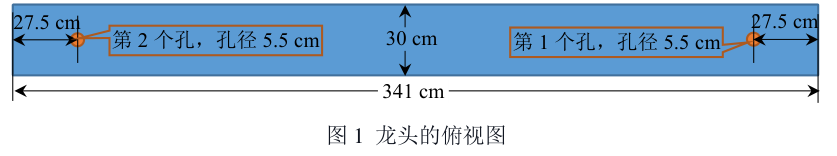
\includegraphics[width=\linewidth]{figures/dragon_statement_fig1.png}
  \caption{Official statement figure (cropped from the CUMCM 2024 A PDF) delivered to the agent.}
  \label{fig:dragon}
\end{subfigure}
\hfill
\begin{subfigure}{0.56\textwidth}
  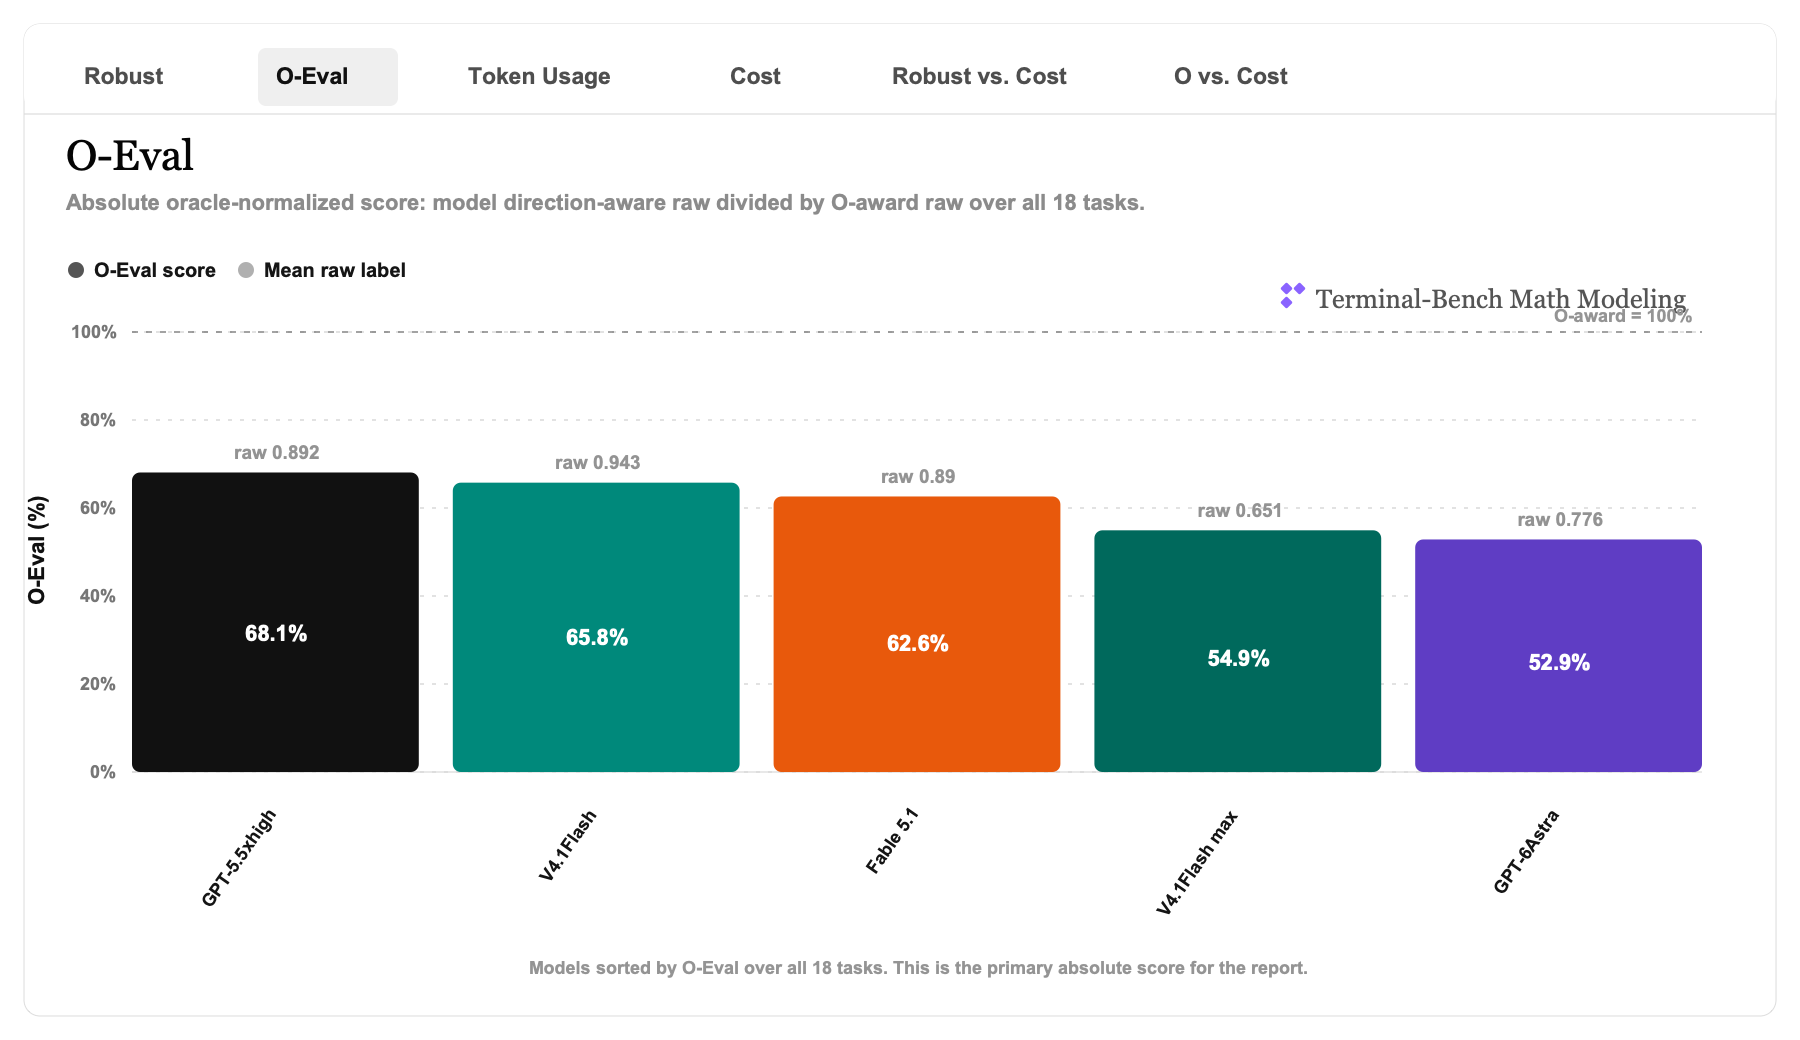
\includegraphics[width=\linewidth]{figures/mm-o-eval-bar.png}
  \caption{\oeval{} for the multimodal subset.}
  \label{fig:bar}
\end{subfigure}
\caption{Left: an official statement figure, cropped from the source PDF and delivered inline in the prompt---one of the 21 load-bearing figures. Right: the multimodal \oeval{} board.}
\label{fig:teaser}
\end{figure}

\section{Limitations, Ethics, and Reproducibility}
\label{sec:limitations}

\paragraph{Anchors are reproductions, not optima.} Every task is normalised against one outstanding paper's reproduction. Different teams make different assumptions, so a low \oeval{} can mean ``different modeling choices'' rather than ``worse modeling''. We mitigate this by one-sided scoring and by excluding demonstrably non-comparable metrics, but the choice of a single anchor is a structural limitation.

\paragraph{Single run; no multi-seed statistics.} All entries use one attempt per task (Section~\ref{sec:setup}). We therefore report single-run numbers, do not select the best run, and cannot report multi-seed mean/std except on the one task with repeated attempts.

\paragraph{Reference scale and scope.} Several anchors report values whose units the schema does not pin (an arbitrary population index; a 0--1 vs.\ 0--100 index). Where the mismatch is provably a unit issue we exclude the metric; where it is a genuine modeling divergence we keep it. Some remaining low scores still reflect the anchor, not the model, and we quantify this (Section~\ref{sec:analysis}) rather than hide it.

\paragraph{Feasibility layers cover A and B, not C.} Both the programmatic gate and the Lean layer check unit/value ranges and internal consistency; they cannot check whether a model's physical claim is true (Section~\ref{sec:abc}). Four constraints that needed an independent replay are handled by hand adjudication, which is not scalable and is a candidate for future automation.

\paragraph{Prompt versioning.} Some trials predate edits to \texttt{instruction.md}; the paper describes the prompt as delivered per the recorded trials. Reproducing today's file would not reproduce those runs exactly.

\paragraph{Ethics: data and licensing.} Problem statements and attachments are official CUMCM/MCM material, used here for research evaluation; we do not redistribute solutions, and the reproduction code is derived from the ``Math-Modeling-BAO'' corpus with per-task provenance recorded (\texttt{paper\_id}, PDF/OCR source). Users of this benchmark should confirm the licence terms of the contest material for their own redistribution.

\paragraph{Reproducibility artefacts.} The repository contains: the task generator, all 18 task directories, the scoring scripts with their contract tests, the feasibility gate with its coverage/discrimination tests, and the Lean project with its generator, discrimination suite, and trust audit. The leaderboard is regenerated by a single documented script; the pricing used for cost is pinned to a fixed snapshot so that costs do not drift between runs.

\section{Conclusion}

We presented \bench{}, a multimodal, artifact-scored benchmark of 18 real mathematical-modeling problems with two distinguishing design choices: \emph{direction-aware, one-sided scoring} that never penalises beating the anchor, and \emph{two-layer feasibility verification} combining a programmatic gate over six decidable invariant forms with 624 kernel-checked Lean obligations.

Across 16 model/harness configurations we find that frontier capability is compressed relative to cost---a \$2.54 model reaches 65.76\% \oeval{} against 68.07\% for a \$99.37 model---that raising a model's thinking tier can hurt, and that most residual failures trace to reference scale and scope rather than to modeling error. We documented several anchor-based scoring pitfalls, repaired the ones that were ours, and quantified which of them actually move the leaderboard. Finally, we showed a case where the benchmark itself was wrong and the models were right, which is the sharpest argument for making feasibility independently checkable.

The two-layer verification design is, we believe, the transferable idea: use a fast programmatic gate to cover every task, and a proof assistant to make the audit's own correctness machine-checkable---while stating plainly the questions (external physical truth, witness completeness) that neither can answer.


\bibliographystyle{plain}
\bibliography{refs}

\appendix
\section{Appendix A: Dataset Details and Split}
\label{app:dataset}

\subsection{Composition}
\bench{} has \textbf{18 tasks}, listed in Table~\ref{tab:tasks} (main text). Composition:
\begin{itemize}[leftmargin=1.4em,itemsep=1pt]
\item \textbf{CUMCM} (Chinese): 2023, 2024, 2025 $\times$ problems A, B, C $=$ 9 tasks.
\item \textbf{MCM} (English): 2023, 2024, 2025 $\times$ problems A, B, C $=$ 9 tasks.
\end{itemize}
Each task is a full contest problem (several sub-questions); only the numeric core of the \emph{final} question is scored (Section~\ref{sec:scoring}). Problem A is typically physical/engineering, B optimization/data, C data-science; taking all three of each year avoids topical cherry-picking.

\subsection{Per-task summary}
\begin{table}[h]
\centering
\small
\caption{Per-task summary. ``\#Fig.'' counts unique figures cropped from the official PDF; ``\#Metric'' the number of scored metrics; ``Final Q'' the sanctioned final question.}
\label{tab:dataset}
\begin{tabular}{@{}lllcc@{}}
\toprule
Slug & Final Q & Source & \#Fig. & \#Metric \\
\midrule
cumcm-2023-a-heliostat-field   & Q3 & CUMCM 2023 A & 2 & 5 \\
cumcm-2023-b-multibeam-lines   & Q4 & CUMCM 2023 B & 8 & 4 \\
cumcm-2023-c-vegetable-pricing & Q4 & CUMCM 2023 C & 0 & 2 \\
cumcm-2024-a-dragon-dance      & Q5 & CUMCM 2024 A & 5 & 2 \\
cumcm-2024-b-production-decision& Q4 & CUMCM 2024 B & 1 & 6 \\
cumcm-2024-c-crop-planting     & Q1 & CUMCM 2024 C & 0 & 2 \\
cumcm-2025-a-smoke-screen      & Q5 & CUMCM 2025 A & 0 & 2 \\
cumcm-2025-b-sic-thickness     & Q3 & CUMCM 2025 B & 2 & 2 \\
cumcm-2025-c-nipt              & Q4 & CUMCM 2025 C & 0 & 2 \\
mcm-2023-a-plant-community     & final & MCM 2023 A & 0 & 3 \\
mcm-2023-b-maasai-mara         & final & MCM 2023 B & 0 & 5 \\
mcm-2023-c-wordle              & final & MCM 2023 C & 2 & 2 \\
mcm-2024-a-lamprey             & final & MCM 2024 A & 0 & 3 \\
mcm-2024-b-submersible-search  & Q4 & MCM 2024 B & 0 & 2 \\
mcm-2024-c-tennis-momentum     & Q5 & MCM 2024 C & 0 & 4 \\
mcm-2025-a-stair-wear          & Q8 & MCM 2025 A & 1 & 3 \\
mcm-2025-b-juneau-tourism      & Q3 & MCM 2025 B & 0 & 6 \\
mcm-2025-c-olympic-medals      & final & MCM 2025 C & 0 & 5 \\
\midrule
\textbf{Total} & & & \textbf{21} & \textbf{61}$^{\dagger}$ \\
\bottomrule
\end{tabular}
\end{table}
$^{\dagger}$62 declared metrics, 61 scored (one weight-0 Wordle metric excluded).

(Counts verified against the repository; the 21 figures are unique after de-duplication, delivered twice---once inline in \texttt{instruction.md} and once under the container \texttt{figures/} path---for 42 files on disk.)

\subsection{Delivered structure}
Each task directory contains: \texttt{instruction.md} (the prompt), \texttt{task.toml} (metadata and limits), \texttt{environment/} (agent Dockerfile + \texttt{data/}), \texttt{tests/} (verifier + scoring config + anchor), and \texttt{solution/} (oracle). Inside \texttt{environment/data/}:
\begin{itemize}[leftmargin=1.4em,itemsep=1pt]
\item \texttt{problem.md} --- statement copy;
\item \texttt{output\_schema.json} --- the required artifact's field/type template (no values);
\item \texttt{source\_manifest.json} --- maps each visible file to its path in the source corpus;
\item \texttt{attachments/} --- verbatim official attachments under flat filenames, with \texttt{INDEX.md};
\item \texttt{repo/} --- the same material at its original nested corpus paths, for reproducibility;
\item \texttt{figures/} --- the cropped figures for the 6 tasks that have them.
\end{itemize}

\subsection{Split}
\textbf{There is no train/validation/test split.} \bench{} is a pure evaluation set: the 18 tasks are all evaluation tasks, evaluated uniformly, with no held-out partition and no per-task difficulty tier. (The repository does contain one in-task \texttt{train\_test\_split} inside a single task's oracle model for the Wordle problem; that is part of that problem's modeling content and is unrelated to benchmark partitioning.)

\subsection{Data sources}
Statements, attachments, and figures derive from the official contest material, mirrored locally via the ``Math-Modeling-BAO'' corpus: CUMCM statements from \texttt{cumcm/problems/\{year\}/\{X\}.md} and MCM from \texttt{mcm/problems/\{year\}/\{X\}.md}. Outstanding-paper PDFs/OCR used for anchors come from the same corpus's \texttt{outstanding/} tree. Every task records its paper id, the PDF/OCR source paths, and its \texttt{reproduction\_scope}.

\section{Appendix B: Software and Hardware Environment}
\label{app:environment}

\subsection{Host and framework}
The evaluation harness is \textbf{harbor 0.14.0}, run from a macOS host (Darwin 25.3, arm64). Harbor orchestrates per-task Docker containers; the enforced resource limits are container limits, not host limits. Task schema version is \texttt{1.3}.

\subsection{Agent container}
All 18 tasks use the same base and dependency set:
\begin{itemize}[leftmargin=1.4em,itemsep=1pt]
\item Base image: \texttt{python:3.12-slim}, plus \texttt{uv} (0.8.15) copied from \texttt{ghcr.io/astral-sh/uv}.
\item OS packages: \texttt{bash}, \texttt{ca-certificates}, \texttt{libgomp1}, \texttt{libgfortran5}, \texttt{tmux}.
\item Python environment at \texttt{/opt/venv}: NumPy 2.0.2, pandas 2.2.2, SciPy 1.14.1, scikit-learn 1.5.2, Matplotlib 3.9.2 (\texttt{MPLBACKEND=Agg}), openpyxl 3.1.5, xlrd 2.0.1.
\item Writable paths: \texttt{/root/data} (read-only inputs), \texttt{/root/results} (the scored artifact), \texttt{/logs/agent}.
\end{itemize}

\subsection{Verifier container}
The verifier runs in a \emph{separate} container (\texttt{environment\_mode="separate"}) built from a minimal \texttt{python:3.12-slim} image installing only \texttt{pytest==8.4.1} and \texttt{pytest-json-ctrf==0.3.5}. It has no network and no access to the agent's working directory beyond the copied artifacts. Verifier timeout is 180~s.

\subsection{Resource limits}
Identical for all tasks: 2 CPUs, 8192~MB memory, 20480~MB storage, 0 GPUs. Build timeout 900~s. Agent timeout 14400~s (4~h), also stated at the end of each prompt. Per-job overrides in the recorded runs set memory to 3072--4096~MB; execution used one concurrent trial and no retries.

\subsection{Network isolation}
Every task sets \texttt{allow\_internet=false}. Model traffic is routed through a local retry proxy (e.g.\ a CLIPROXY endpoint) so that the agent can call the model API but cannot fetch solutions, download packages, or install tooling at runtime. This is what makes the harness install step special: for CLI agents (\texttt{codex}, \texttt{opencode}, \texttt{claude-code}) the client has to be present in the image, since it cannot be installed after the trial starts. The third-party operator's runs did exactly this---pre-installing the CLIs at the end of the Dockerfile and allow-listing only the model gateway, leaving statement, data, and verifier unchanged.

\subsection{Frozen versions}
For reproducibility we note: harbor 0.14.0; task schema 1.3; the Python dependency pins above; the pricing snapshot used for cost is a fixed local file (the board no longer fetches live prices, so costs are stable across reruns).

\section{Appendix C: Experimental Settings}
\label{app:settings}

\subsection{Per-entry configuration}
\begin{table}[h]
\centering
\small
\caption{Per-entry configuration. ``Tier'' is the reasoning setting actually passed to the model.}
\label{tab:app-configs}
\begin{tabular}{@{}lllll@{}}
\toprule
Entry & Model id & Harness & Tier & Multimodal \\
\midrule
codex + gpt-5.5 xhigh        & \texttt{openai/gpt-5.5} & codex CLI & \texttt{reasoning\_effort=xhigh} & yes \\
opencode + deepseek-flash    & \texttt{deepseek/deepseek-v4.1-flash} & opencode CLI & high (default) & yes \\
opencode + deepseek-flash (max) & \texttt{deepseek/deepseek-v4.1-flash} & opencode CLI & \texttt{variant=max} & yes \\
codex + GPT-6 Astra          & \texttt{gpt-6-astra} & codex CLI & max & yes \\
claude-code + Fable 5.1      & \texttt{claude-fable-5-1} & claude-code CLI & max & yes \\
Qwen3.8-27B-FP8 thinking     & \texttt{qwen/qwen3.8-27b} & terminus-2 & thinking & no \\
Tencent Hy4 Preview          & \texttt{tencent/hy4-preview} & terminus-2 & default & no \\
GPT-5.6 SOL high             & \texttt{openai/gpt-5.6-sol} & terminus-2 & high & no \\
GPT-5.6 SOL xhigh            & \texttt{openai/gpt-5.6-sol} & terminus-2 & xhigh & no \\
v4 pro                       & \texttt{deepseek/deepseek-v4-pro} & terminus-2 & default & no \\
GLM-5.3                      & \texttt{z-ai/glm-5.3} & terminus-2 & default & no \\
Kimi K3                      & \texttt{moonshotai/kimi-k3} & terminus-2 & default & no \\
GLM-5.3-Flash (ox-alpha)     & \texttt{z-ai/glm-5.3-flash} & terminus-2 & default & no \\
v4 flash baseline            & \texttt{deepseek/deepseek-v4-flash-0731} & terminus-2 & default & no \\
Qwen3.8 Flash (Bailian)      & \texttt{qwen/qwen3.8-flash} & terminus-2 & default & no \\
Gemini 3.7 Flash high        & \texttt{google/gemini-3.7-flash} & terminus-2 & high & no \\
\bottomrule
\end{tabular}
\end{table}

Multimodal status is defined by which harness exposes an image channel; the 11 \texttt{terminus-2} entries cannot open the cropped PNGs, which is why the multimodal subset (Table~\ref{tab:mm}) is reported separately.

\subsection{Agent command templates}
The task statement is passed to the agent as its prompt. Representative commands (from the recorded \texttt{trial.log}s):
\begin{verbatim}
# codex
codex exec --dangerously-bypass-approvals-and-sandbox --skip-git-repo-check \
  --model gpt-5.5 --json --enable unified_exec \
  -c model_reasoning_effort=xhigh -- '<instruction.md body>'

# opencode
opencode --model=openai/deepseek-flash run --format=json --thinking \
  --dangerously-skip-permissions -- '<instruction.md body>'
\end{verbatim}
\texttt{terminus-2} is driven by harbor, which prepends a generic command-line
system prompt (``Provide batches of shell commands\ldots format your response as
JSON'') and then the statement.

\subsection{Retries, concurrency, and artifact recovery}
All entries used \texttt{n\_concurrent\_trials=1} and \texttt{n\_attempts=1} with
no automatic retries. Two subtleties are disclosed:
\begin{itemize}[leftmargin=1.4em,itemsep=1pt]
\item \textbf{Misfiled artifacts.} Two tasks (lamprey; and, at the max tier, the
same) wrote the result as \texttt{<slug>-result.json} rather than the required
\texttt{<slug>\_result.json} (hyphen vs.\ underscore), so the harness did not
collect it. We replayed the recorded run's scripts to reproduce the artifact and
re-scored it; the reproduction is marked in the report.
\item \textbf{Third-party runs.} The GPT-6 Astra and Fable 5.1 entries were run
by independent operators. Because their verifier used a different reward
formula, we re-scored their saved artifacts with \emph{our} scorer and current
anchors, so that all 16 rows share one scoring definition. Where their artifacts
were not packaged, we reconstructed the scored fields from their saved
per-metric records (verified to reproduce their own numbers exactly on tasks
where the full artifact was present).
\end{itemize}

\subsection{Cost accounting}
Cost is computed from measured token usage against a \emph{fixed} price
snapshot, with two adjustments stated in the report: reasoning tokens that the
provider bills outside its completion counter are added to output; and where a
provider charges a peak/off-peak rate, the peak rate is used. For the two
third-party entries, cost is their own measured per-run USD. Prices are a fixed
local file so that costs do not drift between reruns.

\section{Appendix D: Baseline Information}
\label{app:baselines}

The word ``baseline'' is overloaded in this benchmark; we distinguish three
distinct objects so the numbers are unambiguous.

\subsection{The flash baseline (score normalization)}
\beval{} and \roeval{} are computed against a \emph{single reference submission},
the \texttt{v4 flash baseline} (\texttt{deepseek/deepseek-v4-flash-0731} under
\texttt{terminus-2}). It defines the zero point: \beval{} is the raw gain over
it, and \roeval{} normalises the model--baseline gain by the
oracle--baseline gap. It is a model submission, not a curated baseline panel.

\subsection{The outstanding anchor (score ceiling)}
Each task's ceiling is the reproduction of one O-award paper. This is the value
that scores \oeval{}$=100\%$. Anchors and their paper ids:

\begin{table}[h]
\centering
\small
\caption{O-award anchor per task.}
\label{tab:app-anchors}
\begin{tabular}{@{}llll@{}}
\toprule
Slug & Paper id & Slug & Paper id \\
\midrule
cumcm-2023-a-heliostat-field   & A175    & mcm-2023-a-plant-community    & 2309229 \\
cumcm-2023-b-multibeam-lines   & B226    & mcm-2023-b-maasai-mara        & 2315379 \\
cumcm-2023-c-vegetable-pricing & C050    & mcm-2023-c-wordle             & 2307946 \\
cumcm-2024-a-dragon-dance      & A016    & mcm-2024-a-lamprey            & 2407093 \\
cumcm-2024-b-production-decision& B159   & mcm-2024-b-submersible-search & 2419984 \\
cumcm-2024-c-crop-planting     & C038    & mcm-2024-c-tennis-momentum    & 2401298 \\
cumcm-2025-a-smoke-screen      & A196    & mcm-2025-a-stair-wear         & 2501909 \\
cumcm-2025-b-sic-thickness     & B157    & mcm-2025-b-juneau-tourism     & 2504448 \\
cumcm-2025-c-nipt              & C023    & mcm-2025-c-olympic-medals     & 2505964 \\
\bottomrule
\end{tabular}
\end{table}

Each anchor is a runnable script (\texttt{solution/oracle/}) that reads the
official attachments and emits the artifact JSON, plus a committed
\texttt{expected\_result.json} recording its values. Oracle coverage is 18/18.

\subsection{Legacy per-task baseline endpoints}
Fifteen of 18 tasks use \texttt{legacy\_target\_distance\_to\_outstanding}
scoring with a legacy baseline endpoint; three (\texttt{mcm-2023-c-wordle},
\texttt{mcm-2025-a-stair-wear}, \texttt{mcm-2025-b-juneau-tourism}) use true
per-metric baseline-to-outstanding min--max endpoints. The distinction is
recorded per metric in each \texttt{score\_config.json} and surfaced in the
report's per-task tables.

\subsection{Anchor caveats}
Two anchors carry caveats that affect how their scores should be read:
\begin{itemize}[leftmargin=1.4em,itemsep=1pt]
\item \textbf{\texttt{cumcm-2024-c-crop-planting} is a marked special case.} The
paper's full constraint set is jointly infeasible on the official attachments
and its reported value came from an undisclosed heuristic; the anchor is a
reproducible exact MILP optimum under the paper's per-plot demand cap.
\item \textbf{\texttt{cumcm-2024-a-dragon-dance} was corrected.} The paper's
1.406276~m/s is infeasible (a handle would reach 2.2568~m/s); the anchor is the
continuous-time value 1.246266~m/s, and the metric direction is
\texttt{target\_value}.
\end{itemize}
These are examples of the general principle: an anchor is a reproduction of one
team's choices, and its provenance must be inspectable.

\section{Appendix E: Prompt Design}
\label{app:prompts}

\subsection{The prompt is the task statement}
There is no hand-written prompt wrapper in this benchmark. The prompt is the
task's \texttt{instruction.md}, delivered verbatim by the harness. Its structure
is fixed across tasks:

\begin{enumerate}[leftmargin=1.4em,itemsep=1pt]
\item a machine-readable canary comment (stripped before delivery);
\item \texttt{\# Original Contest Problem} --- the verbatim contest statement,
with each cited figure embedded inline as \texttt{![图 N](fig\_N.png)};
\item any results tables the statement requires, as plain text;
\item \texttt{\# 题面附图} / \texttt{\# Figures} --- a note listing the
in-container figure paths (e.g.\ \texttt{/root/data/figures/fig\_1.png\ldots});
\item \texttt{\# Required Benchmark Artifact} --- instructs the agent to solve
the problem, points at the mirrored attachments, names the required output path,
and points at the output schema;
\item the time limit line (\texttt{You have 14400 seconds\ldots}).
\end{enumerate}

\subsection{The artifact block (verbatim template)}
\begin{verbatim}
# Required Benchmark Artifact

Solve the contest problem above. The official attachments are mirrored at
`/root/data/attachments` (flat filenames; see
`/root/data/attachments/INDEX.md`) and also remain at their full corpus paths
under `/root/data/repo`. Use them whenever they are relevant. Write your final
structured answer to:

/root/results/<slug>_result.json

The result must be valid JSON and should follow the shape shown in
`/root/data/output_schema.json`. Include the numerical quantities, modeling
decisions, diagnostics, sensitivity or uncertainty results, conclusions for the
contest questions, and generated artifact paths needed to support your answer.
You may also write supplementary CSV, XLSX, or PNG files under `/root/results`,
but the JSON file above is the required artifact.

You have 14400 seconds to complete this task. Do not cheat by using online
solutions or hints specific to this task.
\end{verbatim}

\subsection{Harness wrapping}
Three harnesses deliver the same text differently:
\begin{itemize}[leftmargin=1.4em,itemsep=1pt]
\item \textbf{terminus-2} (harbor): prepends a fixed command-line system prompt
(``You are an AI assistant tasked with solving command-line tasks in a Linux
environment\ldots provide batches of shell commands\ldots format your response as
JSON with \texttt{commands:[{keystrokes,duration}]}'') and then appends
\texttt{Task Description:} followed by the statement.
\item \textbf{codex CLI}: the statement is the positional prompt
(\texttt{codex exec \ldots\ -{}- '<statement>'}).
\item \textbf{opencode CLI}: the statement is the positional prompt
(\texttt{opencode run \ldots\ -{}- '<statement>'}).
\end{itemize}

\subsection{Version caveat}
The \texttt{instruction.md} files were revised after some trials were recorded:
a figure-path section was added, and one MCM statement was re-sourced from the
official PDF. The prompt actually delivered in a given trial is the one captured
in that trial's \texttt{trial.log} / \texttt{trajectory.json}; for
reproducibility, cite those, not the current file. This is why we describe the
prompt structure above rather than quoting today's file as if it were what every
model saw.

\subsection{What the prompt does \emph{not} say}
Deliberately, the prompt gives no modeling hints, no method suggestions, and no
pointer to the scored fields beyond the schema. It also does not tell the agent
which sub-question is scored, except that the artifact is required and must
contain ``the numerical quantities\ldots conclusions for the contest questions''.
This keeps the benchmark a test of doing the whole modeling problem, at the cost
of the agent having to infer which numbers matter.

\section{Appendix F: Case Studies (Full Numerics)}
\label{app:cases}

We give the full per-field comparison for the three case studies. Values are read
from each role's saved artifact; the oracle column is the anchor.

\subsection{F.1 Dragon-dance (CUMCM 2024 A, Q5)}
\begin{table}[h]
\centering
\small
\caption{Dragon-dance final question. All three roles agree; the paper value is the outlier and is infeasible.}
\label{tab:case-dragon}
\begin{tabular}{@{}lccc@{}}
\toprule
Quantity & Oracle (anchor) & GPT-5.5 & DeepSeek V4.1 \\
\midrule
\texttt{max\_head\_speed\_mps}        & 1.246266 & 1.24626636 & 1.24626636 \\
\texttt{max\_speed\_ratio}            & 1.604793 & 1.60479338 & 1.60479338 \\
peak time (s)                         & 14.48    & ---        & --- \\
\midrule
\multicolumn{4}{@{}l@{}}{\emph{Paper's isolated value:} 1.406276 m/s (ratio 1.422195) --- infeasible: implies 2.2568 m/s at a handle.} \\
\bottomrule
\end{tabular}
\end{table}

Discussion: the reconstruction of the true peak is a continuous-time maximum of
the handle-speed ratio; the paper sampled integer seconds and stepped over it. The
exact identity \texttt{head\_speed}$\times$\texttt{ratio}$=2$~m/s (checked by both
the programmatic gate and the Lean layer) is what exposes the paper value as
infeasible.

\subsection{F.2 Crop-planting (CUMCM 2024 C, Q1)}
\begin{table}[h]
\centering
\small
\caption{Crop-planting final question (special case: anchor is a reproducible exact optimum under the paper's per-plot cap).}
\label{tab:case-crop}
\begin{tabular}{@{}lccc@{}}
\toprule
Quantity (yuan, 7-year) & Anchor (exact MILP) & GPT-5.5 & DeepSeek V4.1 \\
\midrule
waste-surplus profit   & 40{,}418{,}876.72 & 40{,}320{,}587.0 & 41{,}559{,}514.9 \\
50\%-discount profit   & 58{,}718{,}967.38 & 66{,}485{,}662.3 & 70{,}378{,}275.8 \\
\bottomrule
\end{tabular}
\end{table}

Discussion: the paper's full constraint set is infeasible on the official
attachments, so the anchor is a reproducible MILP optimum; the models' plans sit
in the same regime. Note the anchor is \emph{between} the two models on the
discount column, which is why a single scalar cannot summarise this task.

\subsection{F.3 Juneau tourism (MCM 2025 B, final question)}
\begin{table}[h]
\centering
\small
\caption{Juneau tourism recommended policy. The sustainability score is reported on different unit scales by different agents.}
\label{tab:case-juneau}
\begin{tabular}{@{}lcccc@{}}
\toprule
Quantity & Anchor & GPT-5.5 & DeepSeek V4.1 & Fable 5.1 \\
\midrule
daily cap            & 11{,}000 & 20{,}000 & 16{,}000 & 14{,}000 \\
visitor fee (USD)    & 55       & 20       & 30       & 30 \\
annual visitors      & 1{,}491{,}526 & 1{,}453{,}152 & 1{,}433{,}729 & 1{,}727{,}733 \\
resident acceptance  & 1.0      & 0.743    & 0.938    & 0.696 \\
sustainability score & 1.007    & 0.900    & 0.706    & 79.1 \\
total revenue (USD)  & 431{,}610{,}328 & 369{,}645{,}540 & 366{,}651{,}514 & 458{,}497{,}065 \\
\bottomrule
\end{tabular}
\end{table}

Discussion: this is the clearest scale problem. The anchor is on a $\sim$1 unit
scale; one third-party agent reports the same field on a 0--100 ``multiattribute
utility'' scale (a scale it explicitly declares in its own artifact). The task's
output schema does not pin the range, so the agent is not wrong---which is why the
correct repair is to specify the field's range in the schema, not to rescale in
the scorer.

\section{Appendix G: Scoring Details}
\label{app:scoring}

\subsection{The metric panel}
Every task ships a \texttt{tests/score\_config.json} declaring its scored metrics.
A metric entry specifies: \texttt{path} (dot/index path into the artifact),
\texttt{oracle\_value}, optional \texttt{baseline\_value}/\texttt{outstanding\_value},
\texttt{direction} (and a matching \texttt{semantic\_direction}),
\texttt{normalization\_mode}, and \texttt{weight}. Across the 18 tasks there are
\textbf{62 declared metrics}, of which \textbf{61 are scored} (one Wordle metric declares weight~0 and is recorded but excluded from the panel); the per-task counts are in Table~\ref{tab:dataset}.

\subsection{Formulas}
Let $R$ be a submission's weighted panel raw, $F$ the flash baseline's, $O$ the
oracle's, and $\mathrm{gain}=R-F$, $\mathrm{gap}=O-F$:
\[
\oeval = \mathrm{clamp}\!\left(\frac{R}{O},0,1\right), \qquad
\beval = R - F, \qquad
\roeval =
\begin{cases}
\mathrm{clip}\!\left(\frac{\mathrm{gain}}{\mathrm{gap}},-1,1\right), & \mathrm{gap}\ge0.10,\\[3pt]
\mathrm{clip}\!\left(\mathrm{gain},-0.10,0.10\right), & \text{otherwise}.
\end{cases}
\]
A missing or non-scoreable artifact gets $\roeval=-1$. Per-metric reward is given
in Section~\ref{sec:per-metric}; the one-sided property (meeting/beating the
anchor never scores below 1.0) is locked by a contract test.

\subsection{Excluded metrics}
Two metrics are excluded from the panel for every model \emph{and} the oracle,
both by configuration-only rules:
\begin{itemize}[leftmargin=1.4em,itemsep=1pt]
\item the Olympic 4th recommendation
(\texttt{great\_coach\_model.recommendations[3]...}) --- the prompt asks for three
countries; the reproduction emits four rows;
\item the two lamprey raw population indices
(\texttt{final\_parasite\_index}, \texttt{host\_fish\_index}) when
$|O|>5$ --- the anchor is an arbitrary raw index with no schema-pinned unit.
\end{itemize}
Out-of-domain values (correlations outside $[-1,1]$, unit-interval quantities
outside $[0,1]$, negative counts, non-positive physical quantities) are not
excluded but have their reward set to zero, with the reason recorded.

\subsection{Hard-gate decisions}
Seven whole-task penalties were applied across the 16 entries; the reasons are:
four heliostat violations (rated power below 60~MW, or a mirror below the 2~m
minimum), one smoke-screen plan failing an independent coverage replay, one
Juneau answer with unit-invalid acceptance/sustainability values, and one Olympic
answer with a degenerate coach-effect result. Full rows are in the generated
report's ``Hard Gate Decisions'' table.

\subsection{Degenerate-band and validity rules}
The band-widening rule (Section~\ref{sec:edge-rules}) applies to the endpoint
metrics of the three endpoint-style tasks. Applying all scoring fixes in this
paper moved \emph{every} entry upward by 0.05--2.62\,pp, because the affected
penalties applied to all submissions equally---the diagnostic signature of a
systematic scoring error rather than a model difference.

\subsection{Ranking tables}
The generated report
(\texttt{terminus2-direction-aware-flash-baseline-bbo-2023-2025.md}) contains, in
addition to the overall mean and the tempered hard-gated board: year splits,
CUMCM/MCM suite splits, the per-task values, the saturated-gap cases, the hard-gate
decisions, and the price table. Those tables are the machine-generated source for
every number in the main text.

\section{Appendix H: Lean Obligation Catalogue}
\label{app:lean}

\subsection{Per-task obligation counts}
The generator emits one obligation per checkable field; the totals by task are:

\begin{table}[h]
\centering
\small
\caption{Obligations per task (624 total across 18 tasks). ``Skipped'' obligations were reported as missing evidence rather than silently satisfied.}
\label{tab:lean}
\begin{tabular}{@{}lcclc@{}}
\toprule
Task & Oblig. & Skipped & Task & Oblig. \\
\midrule
cumcm-2023-a-heliostat-field   & 12  & 0 & mcm-2023-a-plant-community   & 66 \\
cumcm-2023-b-multibeam-lines   & 3   & 1 & mcm-2023-b-maasai-mara       & 17 \\
cumcm-2023-c-vegetable-pricing & 7   & 0 & mcm-2023-c-wordle            & 3 \\
cumcm-2024-a-dragon-dance      & 3   & 0 & mcm-2024-a-lamprey           & 302 \\
cumcm-2024-b-production-decision& 61 & 0 & mcm-2024-b-submersible-search& 8 \\
cumcm-2024-c-crop-planting     & 5   & 0 & mcm-2024-c-tennis-momentum   & 7 \\
cumcm-2025-a-smoke-screen      & 10  & 0 & mcm-2025-a-stair-wear        & 6 \\
cumcm-2025-b-sic-thickness     & 4   & 0 & mcm-2025-b-juneau-tourism    & 12 \\
cumcm-2025-c-nipt              & 16  & 0 & mcm-2025-c-olympic-medals    & 82 (1 skipped) \\
\bottomrule
\end{tabular}
\end{table}

Four skipped obligations are visible in the generator output: one missing overlap
field (multibeam), four scenarios whose declared grid count is null (maasai
partition), and one recommendation-count interpretation difference (Olympic).

\subsection{Representative obligations}
Over the invariant library, a task supplies bounds and the obligations are
generated. Examples:
\begin{verbatim}
-- domain/range: a rate must lie in [0,1] (scaled x1000)
example : (0 <= 43 /\ 43 <= 1000) := by decide

-- ordering: q95 must not fall below the mean
example : (posterior_mean <= posterior_q95) := by ...

-- exact identity: head_speed * ratio = 2 m/s (scaled)
example : (1980000 <= 1246266 * 1604793 /\ 1246266 * 1604793 <= 2020000) := by decide

-- finite domain: count of decision bits is 16 or 17
example : (len = 16 \/ len = 17) := by decide
\end{verbatim}
Every generated obligation is annotated with the JSON path it came from, so a
reviewer can trace each claim back to the artifact.

\subsection{Trust audit (verbatim excerpt)}
\begin{verbatim}
'Feasibility.atMost_trans'                depends on axioms: [propext, Quot.sound]
'Feasibility.atLeast_mono'                depends on axioms: [propext, Quot.sound]
'CropPlanting.ua_feasible'                does not depend on any axioms
'CropPlanting.ua_in_interpretation_gap'   does not depend on any axioms
'Juneau.ua_acceptance_percent_only'       does not depend on any axioms
'Juneau.ua_sustainability_out_for_any_sane_tol'
                                          depends on axioms: [propext, Quot.sound]
'JuneauSensitivity.reported_infeasible'   depends on axioms: [propext, Quot.sound]
\end{verbatim}
Only \texttt{propext} and \texttt{Quot.sound} (Lean's standard classical logic)
appear, or no axioms at all. No \texttt{sorryAx}, no \texttt{Lean.ofReduceBool}
(i.e.\ no \texttt{native\_decide}); the pipeline greps for both.

\subsection{Discrimination suite}
\texttt{negative\_test.py} mutates one numeric leaf at a time and requires the
build to fail \emph{and} to cite the mutated field. Ten mutations across the six
forms are covered (out-of-range probability, out-of-range correlation, reversed
ordering, violated exact identity, non-positive thickness, reversed interval,
non-binary decision bit, negative acceptance index, $q_{95}$ below mean, zero
species count). All ten are rejected; the suite exits non-zero if any is not.

\subsection{Reproducing the layer}
\begin{verbatim}
export PATH="$HOME/.elan/bin:$PATH"     # Lean 4 via elan
cd lean-feasibility-demo
./verify.sh        # generate -> kernel check -> audit -> discriminate -> references
\end{verbatim}
Toolchain: \texttt{leanprover/lean4:v4.22.0}. No Mathlib; clean build under a
second. The generator also runs against the committed O-award references
(326 obligations, 1 skipped), so the layer can be exercised without the saved
agent artifacts.


\end{document}
